% The Gaussian Case
\section{MROC Surface  under Gaussian Hypotheses}
In the next example we compute the MROC surface under Gaussian Hypotheses. 
Assume three hypotheses given as:
\begin{equation}
\label{equ: Gaussian Hypothesis}
\begin{split}
	H_0:\;\;\;\;\;\;\;\;&X \sim \mathcal{N}(-1,1)\\
    H_1:\;\;\;\;\;\;\;\;&X \sim \mathcal{N}(0,1)\\
    H_2:\;\;\;\;\;\;\;\;&X \sim \mathcal{N}(1,10)\,,
\end{split}
\end{equation}
where $\mathcal{N}(\mu,\sigma^2)$ denotes a Gaussian PDF with mean $\mu$ and variance $\sigma^2$.
To form the M-ROC surface, we first consider points in region $M_0$.The decision rule in region $M_0$ is given by \eqref{equ: decision rule}
with $M=2,\;\;k_1, k_2 \geq 0$, and the expression for $P_d$, $P_{f_1}$ and $P_{f_2}$ are given by \eqref{equ: pf and pd}. According to \textbf{Neyman Pearson Lemma}, if $k_1, k_2 \geq 0$, then $P_{f_1} = c_1$ and $P_{f_2} = c_2$.
We use Matlab to illustrate the region $M_0$. The values of $k_1$ and $k_2$ range from $0$ to $100$ in steps of $0.01$. Substituting the value of $k_1$ and $k_2$ into \eqref{equ: pf and pd}, results in the corresponding $P_d$ $P_{f_1}$ and $P_{f_2}$.  The set $M_0$ is illustrated in Figure \ref{pic: surface for m0 gaussian}. Figure \ref{pic: contour for m0 gaussian} presents the projection of Figure \ref{pic: surface for m0 gaussian} on the $c_1, c_2$ plane.


\begin{figure}[!t]
\centering
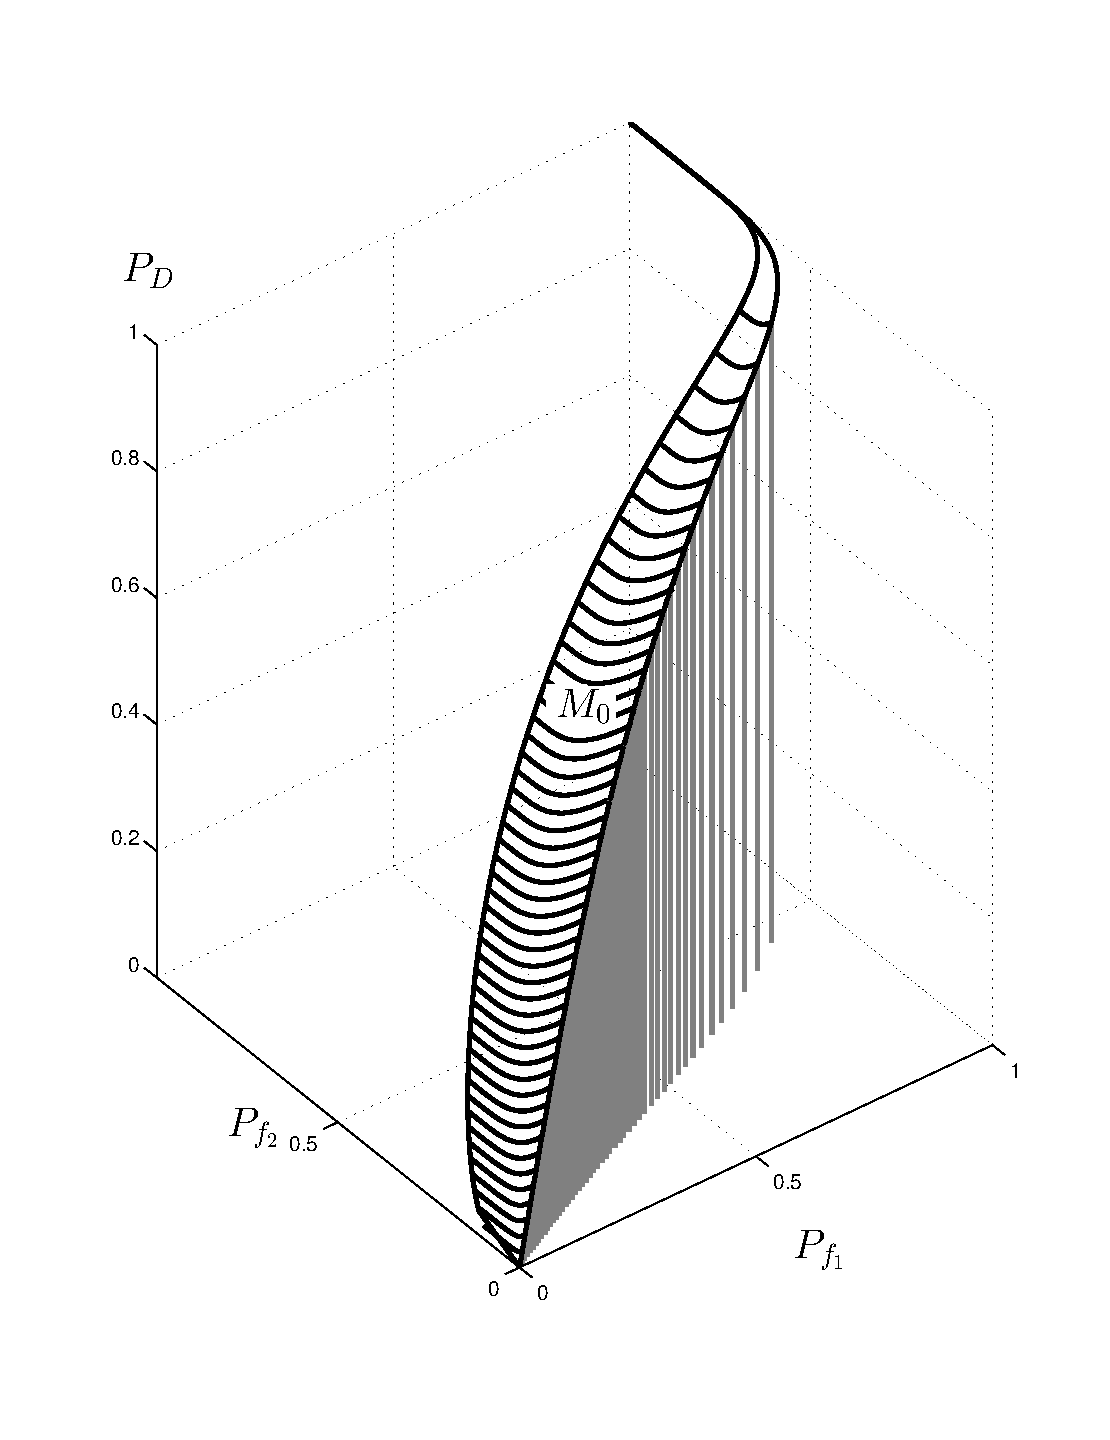
\includegraphics[width=12cm]{3/singleROC.eps}
\caption{Region that can be achieved by Neyman Pearson testing with $k_i \geq 0 (i=1, ..., M)$.}
\label{pic: surface for m0 gaussian}
\end{figure}
\newpage

\begin{figure}[!t]
\centering
\includegraphics[width=12cm]{3/singlecontour.eps}
\caption{Region that can be achieved by Neyman Pearson testing with $k_i \geq 0 (i=1, ..., M)$.}
\label{pic: contour for m0 gaussian}
\end{figure}

In Figure \ref{pic: contour for m0 gaussian}, region $N_0$ is the projection of region $M_0$ on the $c_1, c_2$ plane. Since $M_0$ is the set of points with $[c_1, c_2] \in \alpha^+$, $N_0$ is the region of points that belong to $\alpha^+$.
Define curve $L_1$ as the set of points that satisfy the conditions: (1) $(c_1, c_2) \in N_0$; (2) $(c_1, c_2+\epsilon) \notin N_0$, for any $\epsilon \geq 0$. Define curve $L_2$ as the set of points that satisfy the conditions: (1) $(c_1, c_2) \in N_0$; (2) $(c_1 + \epsilon, c_2) \notin N_0$, for any $\epsilon \rightarrow 0$.
$N_1$ denotes the region enclosed by line $c_1 = 0$, $c_2$; line $c_1$, $c_2 = 1$ and curve $L_1$.
$N_2$ denotes the region enclosed by line $c_1 = 1$, $c_2$; line $c_1$, $c_2 = 0$ and curve $L_2$.
The regions of $N_0$ $N_1$ and $N_2$ are shown in Figure \ref{pic: contour for m0 gaussian}.

\textbf{Conclusion 1}
\textit{\\(1) All points belonging to region $N_1$ or curve $L_1$, if they have the same $c_1$, they have the same decision rule and same $P_d$.
\\(2) All points belonging to region $N_2$ or curve $L_2$, if they have the same $c_2$, they have the same decision rule and same $P_d$.
}

\noindent \textbf{PROOF}

First we prove $F\mathbf{a}$ is a non-decreasing function of $\mathbf{a}$ when $\mathbf{a} \in \alpha^+$.

Since when $\mathbf{a} \in \alpha^+$ we have 
\begin{equation}
\begin{split}
\max_{\mathbf{a}\in \alpha^+}\;\;\;\;&P_d = F(\mathbf{a})\\
\text{s.t.}\;\;\;\;&\mathbf{P}_f = \mathbf{a}
\end{split}
\end{equation}
According to ENP Lemma, $F(\mathbf{a})$ also satisfies
\begin{equation}
\begin{split}
\label{equ: MENP2}
\max_{\mathbf{a}\in \alpha^+}\;\;\;\;&P_d = F(\mathbf{a})\\
\text{s.t.}\;\;\;\;&\mathbf{P}_f \leq \mathbf{a}
\end{split}
\end{equation}
In \eqref{equ: MENP2} when one of $a_i,\;\; i = 1, 2, ..., M$ increases and other $a_i$ remain the same, the constraints become more relax, hence $P_d$ will not decrease. Therefore $F(\mathbf{a})$ is a non-decreasing function of $\mathbf{a}$ when $\mathbf{a} \in \alpha^+$. 
Consider points in region $N_1$. Since $(c_1, c_2) \notin N_0$, we use MENP (\rmnum{2}) to achieve $P_d$. As it is shown in Figure \ref{pic: contour for m0 gaussian}, $A$ is a point in $N_1$ with coordinate $(x, y)$. According to MENP (\rmnum{2}), $\mathcal{C}$ is the set of points lie in region enclosed by curve $L_1$ $L_2$ and line $c_1 = x$. For all points belongs to $\mathcal{C}$, point $B$ has the largest $c_1$ and $c_2$ value. As we proved function $F(c_1, c_2)$ is non-decreasing, point $B$ has the largest $P_d$ among all points belong to region $\mathcal{C}$. Hence we proved point $A$ and point $B$ have the same decision rule and same $P_d$. Since point in region $N_1$ with $c_1 = x$ has the same decision rule and $P_d$ with point $B$, we can conclude: for points belong to region $N_1$ or curve $L_1$, if they have the same $c_1$ value, they have the same decision rule and same $P_d$.

In the same way, we can prove: For points belong to region $N_2$ or curve $L_2$, if they have the same $c_2$ value, they have the same decision rule and same $P_d$.

Q.E.D

Since we already know $P_d$ for points in region $N_0$ and curves $L_1$ and $L_2$ belong to $N_0$, we can get $P_d$ for points in $N_1$ and $N_2$. M-ROC surface for this example is given in Figure  \ref{pic: LJS} and the contour of M-ROC surface is given in Figure \ref{pic: LJS contour}.

\begin{figure}[!t]
\centering
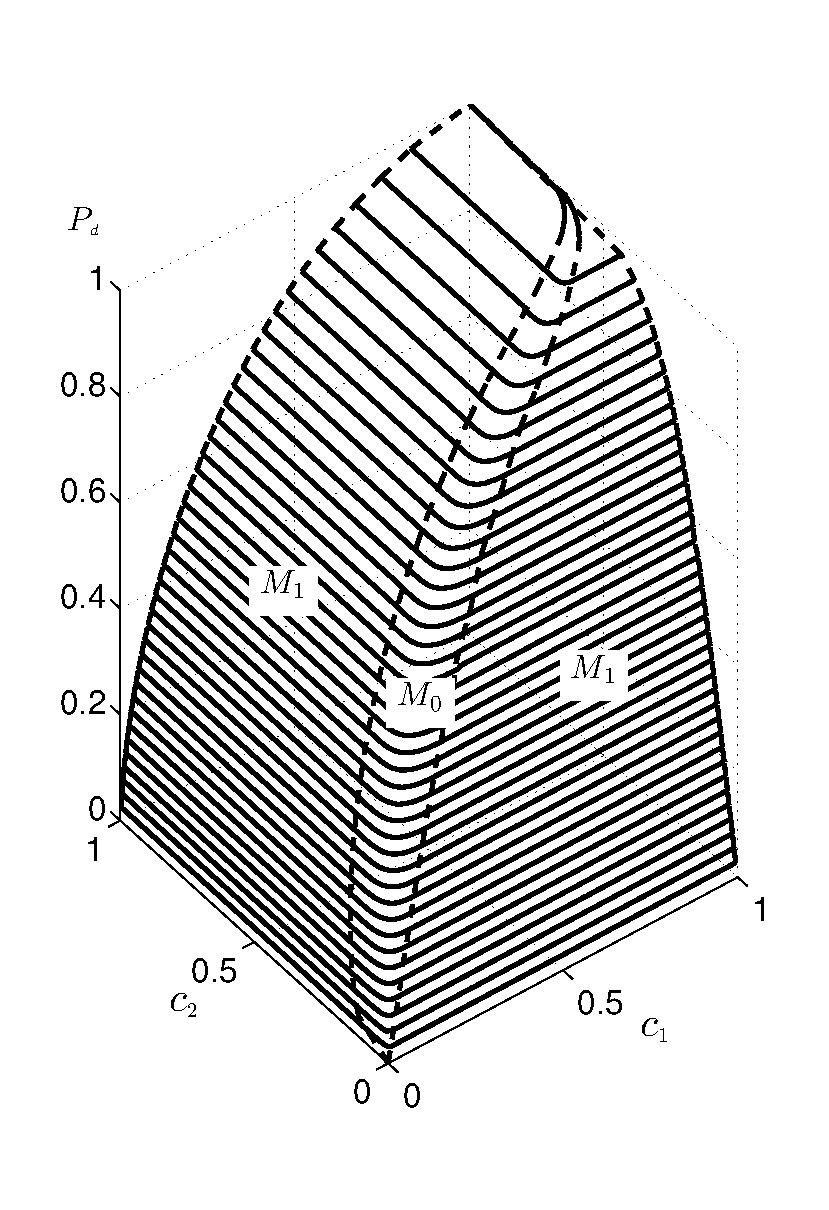
\includegraphics[width=12cm]{3/ROC2.eps}
\caption{The M-ROC surface for Gaussian Hypotheses.}
\label{pic: LJS}
\end{figure}

\begin{figure}[!t]
\centering
\includegraphics[width=12cm]{3/LJcontour.eps}
\caption{Contour for M-ROC surface.}
\label{pic: LJS contour}
\end{figure}

Next we consider a more general case of $M+1$ hypotheses given as
\begin{equation}
\label{equ: m+1 Gaussian Hypo}
\begin{split}
H_0:\;\;\;\;\;\;&X\sim \mathcal{N}(\mu_0, \sigma_0^2)\\
H_1:\;\;\;\;\;\;&X\sim \mathcal{N}(\mu_1, \sigma_1^2)\\
  ......\\
H_M:\;\;\;\;\;\;&X\sim \mathcal{N}(\mu_M, \sigma_M^2)
\end{split}
\end{equation}
We will prove when $\sigma_0^2 = \sigma_1^2 = ... = \sigma_M^2$ and $\mu_0 < \mu_i (i = 1, ..., M)$, the region achieved by ENP test with $k_i \geq 0 (i = 1, ..., M)$ degenerates to a curve.

Consider
\begin{equation}
\label{equ: define gx}
g(x) = \sum_{i=1}^{M}k_i\frac{f_i(x)}{f_0(x)}.
\end{equation}
Since 
\begin{equation}
\label{equ: gaussian PDF}
f_i(x) = \frac{1}{\sqrt{2\pi\sigma_i^2}}\exp(-\frac{(x-\mu_i)^2}{2\sigma_i^2}).
\end{equation}
we have
\begin{equation}
\label{g00}
g(x) = \sum_{i=1}^{M}\frac{\frac{1}{\sqrt{2\pi\sigma_i^2}}\exp(-\frac{(x-\mu_i)^2}{2\sigma_i^2})}{\frac{1}{\sqrt{2\pi\sigma_0^2}}\exp(-\frac{(x-\mu_0)^2}{2\sigma_0^2})}
\end{equation}
Using the condition $\sigma_i^2 = \sigma_0^2 (i = 1, ..., M)$ in \eqref{g00}, we have 
\begin{equation}
\label{equ: gx cc}
g(x) = \sum_{i=1}^{M}k_i\exp(\frac{(\mu_i - \mu_0)(2x-\mu_i - \mu_0)}{2\sigma_0^2})
\end{equation}
Defining $c_i = \frac{\mu_i - \mu_0}{2\sigma_0^2}$, \eqref{equ: gx cc} can be written as
\begin{equation}
g(x) = \sum_{i=1}^{M}k_i\exp(c_i(2x-\mu_0 - \mu_i)
\end{equation}
From the condition $\mu_0 < \mu_i (i=1, ..., M)$, we know $c_i >0$. Hence it can be conclude that $g(x)$ is a monotonically increasing function with $x$. Hence from \textbf{Property 1} we have that the region $M_0$ (region achieved by ENP test with $k_i \geq 0 (i=1, ..., M)$) degenerates to a curve.
For a specific $\mathbf{c}$, the decision rule is 
\[
x \substack{H_0 \\ \leq \\ > \\ \bar{H}_0} x_0
\]
where $x_0 = \min\{F_1^{-1}(c_1), ..., F_M^{-1}(c_M)\}$.
